\documentclass[a4paper,11pt]{article}
\usepackage[utf8]{inputenc}
\usepackage{polski}
\usepackage[polish]{babel}
\let\babellll\lll
\let\lll\relax

\usepackage{graphicx}    % Pakiet pozwalaj¹cy ,,wklejaæ'' grafikê...
\usepackage{caption}
\usepackage{subcaption}
\usepackage{epstopdf}
\usepackage{amsmath,amssymb,amsfonts,amsthm,mathtools}
                               % Do³¹czamy zestaw ró¿nych przydatnych znaczków ...

\usepackage{url}

%\usepackage{comment}  
%\usepackage[left = 2.5cm]{geometry}
\usepackage{bbm}               % \mathbbm{N} - zbior liczb naturalnych
%tikz

\begin{document}

\section{\LARGE{Języki i automaty}}

\textbf{Zadanie 40} \\ \\
Odp: NIE. \\


\begin{figure}[h!]
  \centerline{%
    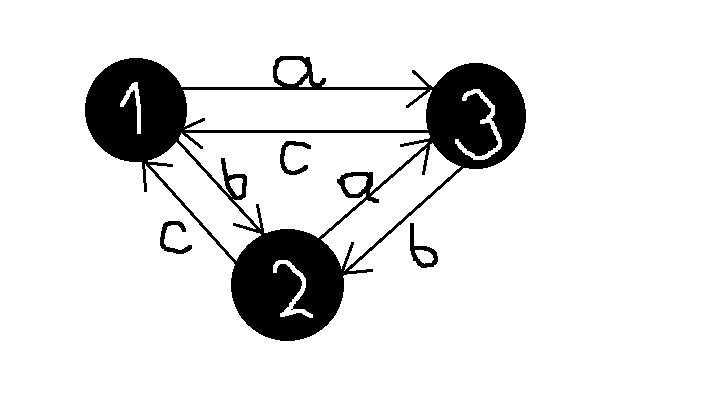
\includegraphics[width=6cm]{zad40.png}%
  }%
  \caption{$csync(\{1,2\}) \supset \{a\}; \ csync(\{1,3\}) \supset \{b\};\ csync(\{1,2\}) \supset \{c\}$. Natomiast $csync(Q) = \emptyset $.}
\end{figure}


\textbf{Zadanie 41} \\ \\
W obydwu podpunktach wystarczy zbadać funkcję

\begin{align*}
 F :\ &2^Q \times \Sigma \longrightarrow 2^Q \\
 F(S,a) &= \{ \delta(q,a) : \ q \in S \}.
\end{align*}

Oczywiście $s \in csync(S) \Longleftrightarrow |\widehat{F}(S,s)| = 1$, gdy zdefiniujemy $\widehat{F}$ w naturalny sposób. 
Ponadto $1 \leqslant |F(A,a)| \leqslant |A|$, zatem $1 \leqslant |\widehat{F}(S,p)| \leqslant |S|$ dla dowolnego prefiksu $p$ słowa $s$,
czyli $\widehat{F}(S,p)$ może przyjmować co najwyżej $\displaystyle{\sum\limits^{|S|}_{k=1}\binom{|Q|}{k}}$ różnych wartości.
Oznaczmy tę liczbę jako $M$. \\ \\

Dla $|s| > M$ istnieją prefiksy $p_1$ i $p_2$ słowa $s = p_1s_1 = p_2s_2, \ |p_1| < |p_2|,$ takie że 
$\widehat{F}(S,s_1) = \widehat{F}(S,s_2)$ (Zasada Szufladkowa). Wtedy oczywiście $\widehat{F}(S,s) = \widehat{F}(S,p_1s_2)$, przy czym 
$|p_1s_2| < |s|$. \\ \\
W zwiazku z powyższym $csync(Q) \neq \emptyset \Longleftrightarrow \exists s \in S |s| \leqslant M$. \\
Dokładne odpowiedzi wynikają z tego wprost, po podstawieniu za $S$ a) dowolniego trzyelementowego zbioru stanów b) Q. \\ \\

\textbf{Zadanie 42} \\ \\
Wystarczy rozwiązać M, L i XL wynikają w prosty sposób. Wskazówka jest myląca. \\ \\

Zbudujmy automat (częściowy) z trzech cykli, ułożonych jeden nad drugim, każdy długości m. Trzy stany, ułożene jeden nad
drugim, będą stanowiły nasz początkowy zbiór S \\ \\

\begin{figure}[h!]
  \centerline{%
    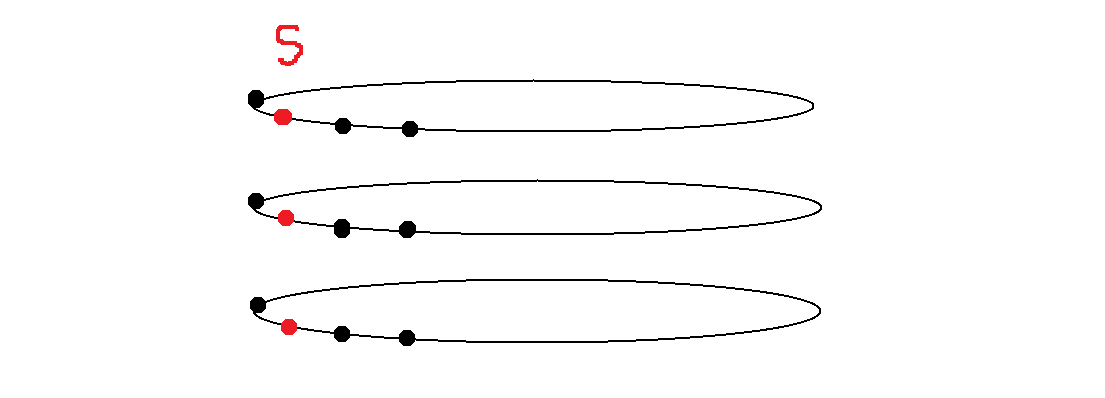
\includegraphics[width=18cm]{zad42.png}%
  }%
\end{figure}

Naszym celem jest, aby co jedną literę zmieniał się stan na górnym cyklu, co $m$ liter stan na drugim, a co $m^2$ na trzecim.
Zapenimy też, że synchronizacja będzie mogła nastąpić dopiero po przejściu przez dolny stan całego cyklu (czyli $~m^3$ krokach). \\
Możemy to wymusić w następujący sposób: \\

\begin{figure}[h!]
  \centerline{%
    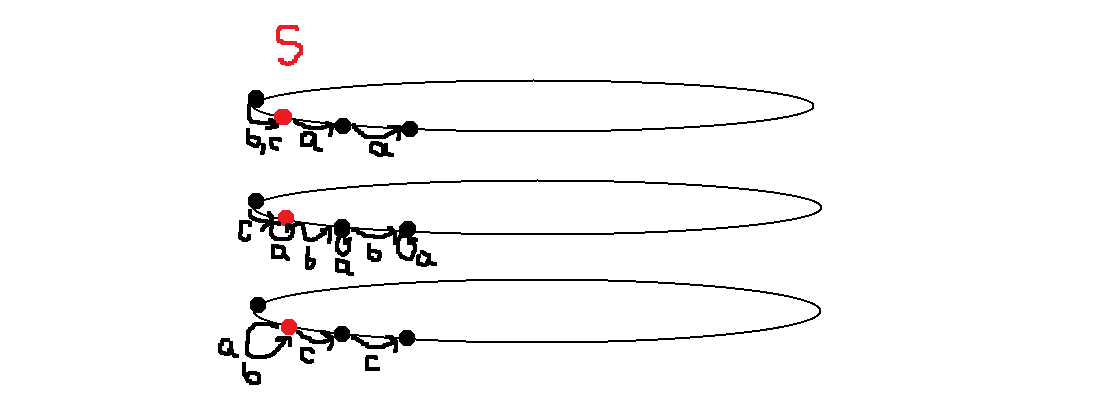
\includegraphics[width=18cm]{zad42_2.png}%
  }%
\end{figure}

przy czym pętelki z literą a są przy każdym stanie na drugim dysku, a pętelki z literami a,b są przy każdym stanie na trzecim
dysku. \\
Możliwość synchronizacji zapeniamy przez dodanie przejść z przedostatnich stanów na każdym dysku do pierwszego stanu 
dolnego dysku. Oznaczenie ich specjalną ``literką synchronizacji'', jak d, zapewni nam, że skorzystać z niej będzie można
dopiero gdy dolny stan dojdzie do przedostatniego miejsca na dolnym dysku (co następuje dopiero po $~m^3$ krokach: \\
\begin{figure}[h!]
  \centerline{%
    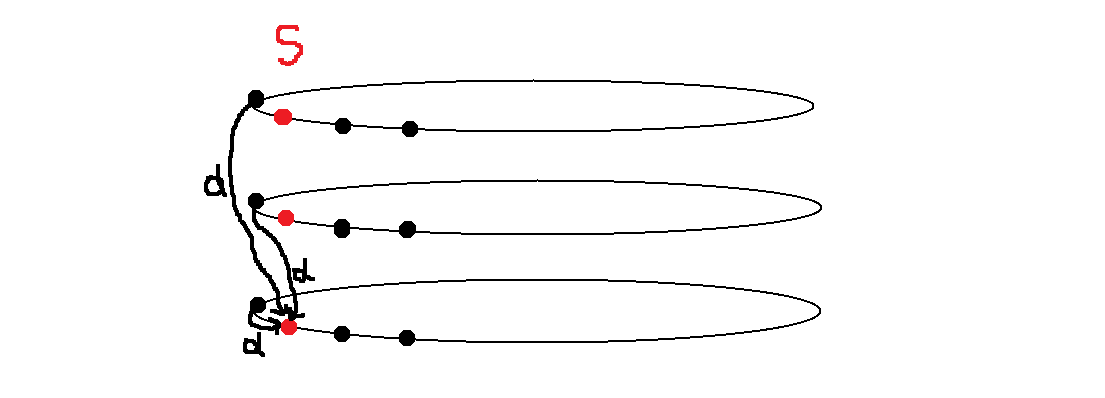
\includegraphics[width=18cm]{zad42_3.png}%
  }%
\end{figure}

Zauważmy teraz, że ten automat (zanim dojedzie do synchronizacji) jednoznacznie wyznacza słowo, dla którego funkcja przejścia 
jest określona dla wszystkich stanów z $S$:
$$
s = ((a^{m-1}b)^{m-1}c)^{m-1}d
$$
Takie $s$ synchronizuje $S$ i nie istnieje żadne krótsze od niego. Nietrudno wyliczyć, że jest ono odpowiednio długie. \\ \\

Co do wersji L i XL, wystarczy zauważyć, że:
\begin{enumerate}
 \item To samo rozumowanie można zastosować dla dowolnie wielu cyki, otrzymując wielomian dowolnie dużego stopnia.
 \item Potrzebny nam alfabet, który ma $k+1$ liter (gdzie $k$ jest liczbą cykli). Ale dowolny alfabet można zamienić na
 dwu(trzy)literowy, zapisując jego litery w systemie bi(try)narnym. Każdy stan trzeba zamienić na stałą liczbę stanów, które 
 wczytają odpowiednią liczbę 0 i 1 (i 2), i w ten sposób będą udawały, że wczytają jedną z naszych $k+1$ liter. Wymaga to około
 $~k$ stanów, ale to tylko stała.
\end{enumerate}

Dodatkowo, dodając pętle z literką przejścia na przedostatnich stanach każdego cyklu, zamienimy nasz automat na taki, który
synchronizuje wszystkie stany ( pierwszy stan każdego cyklu ``zjada'' wszystkie kolejne w pierwszym przejściu cyklu):
\begin{figure}[h!]
  \centerline{%
    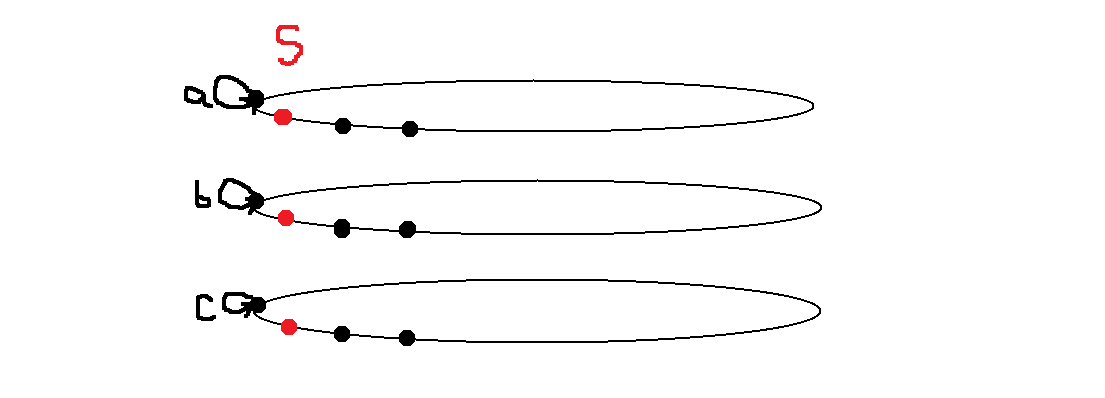
\includegraphics[width=18cm]{zad42_4.png}%
  }%
\end{figure}


\end{document}
